\section{Durchführung}
\label{sec:Durchführung}

Zur Messung wird die in Abbildung \ref{fig:geraet} dargestellte Apparatur verwendet.
Dabei ist das Gerät an einen Computer angeschlossen und die nötigen Einstellungen
können an diesem vorgenommen werden.

\begin{figure}
  \centering
  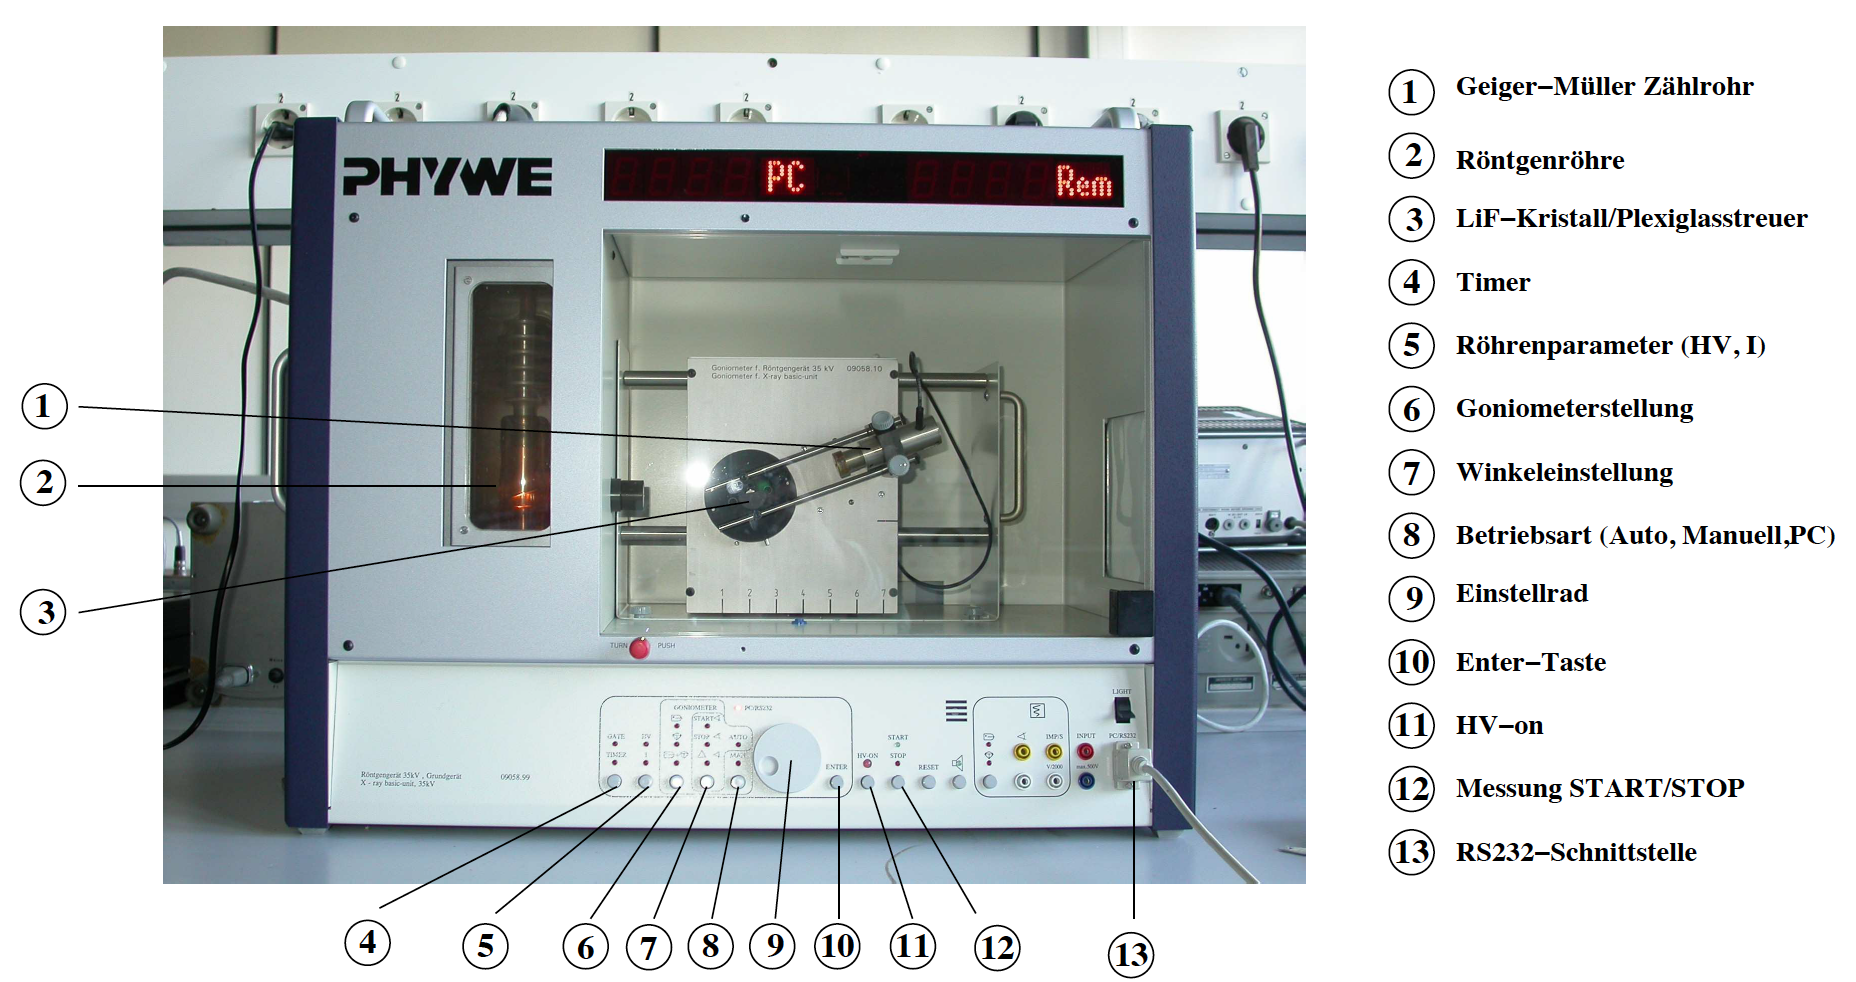
\includegraphics[height=8cm]{data/geraet.png}
  \caption{Foto des verwendeten Geräts mit Beschriftung \cite{Versuchsanleitung}.}
  \label{fig:geraet}
\end{figure}

Für alle Messreihen wird eine Beschleunigungsspannung von $U=35\,$keV und ein
Emissionsstrom von 1\,mA verwendet.

Zuerst soll eine Messreihe zur Überpüfung der Bragg-Bedingung aufgenommen werden.
Dafür wird bei einem festen Kristallwinkel von $\theta=14°$ die Intensität der
Röngenstrahlung in einem Winkelbereich von 26° bis 30° gemessen.

Daraufhin wird das Emissionsspektrum der Röntgenröhre aufgenommen. Dafür muss eingestellt
werden, dass die Messung stets beim Glanzwinkel erfolgt; dass also das Geiger-Müller-Zählrohr
immer dem doppelten Winkel wie der LiF-Kristall hat. Gemessen wird hier in einem
Winkelbereich von 4° bis 26°.

Anschließend werden die Absorptionsspektren um die K-Kante herum für vier verschiedene
Elemente mit Ordnungzahlen zwischen $Z=30$ und $Z=50$ gemessen. Der Winkelbereich wird
dabei abhängig von dem Theoriewert für die K-Kanten der Elemente gewählt.

Abschließend wird das Absorptionsspektrum um die L-Kante von Gold herum gemessen.
Der Winkelbereich wird hier ebenfalls entsprechend des Theoriewerts für die
L-Kante gewählt.
